\chapter{Аналитическая часть}

В данном разделе рассматривается система, в которой происходит волновой процесс, состоящая из поверхности воды и предмета. Изучаются и сравниваются методы и алгоритмы, визуализирующие волны. В результате анализа определяется алгоритм, эффективно решающий задачу моделирования волн, образованных движением объекта.

\section{Волновой процесс}

Процесс образования волны при условии, что частицы воды находятся в состоянии равновесия, состоит из следующих этапов:

\begin{itemize}
	\item на поверхность воды оказывается внешнее воздействие (ветер, движение корабля, падение камня), частицы жидкости опускаются вниз, водная поверхность становится вогнутой;
	\item сила тяжести или сила поверхностного натяжения стремятся вернуть частицы в состояние равновесия;
	\item частицы воды переходят положения равновесия, и поверхность воды становится выпуклой.
\end{itemize}

Движение передается от одних частиц к другим. Этапы волнового процесса показаны на рисунке \ref{img:wave-process}.

\begin{figure}[H]
	\begin{center}
		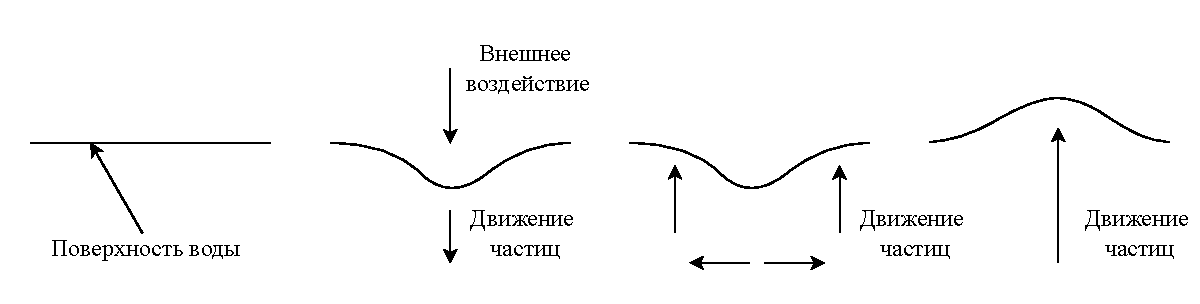
\includegraphics[scale=0.8]{img/wave-process.pdf}
	\end{center}
	\captionsetup{justification=centering}
	\caption{Процесс образования волны}
	\label{img:wave-process}
\end{figure}

Если восстановить равновесие стремится сила тяжести, то волны называются гравитационными, если сила поверхностного натяжения --- капиллярными. Волны называют капиллярно-гравитационными, когда силы сопоставимы.

\section{Модели предмета и волны}

Механизм образования волн подчиняется закону дисперсии. Дисперсия волн --- это зависимость скорости распространения волн от их частоты. Именно дисперсия создает сложную картину волн, образованных телом в воде.

\subsection{Модель предмета}

Внешним воздействием в моделируемой системе является движение предмета. Для правильной обработки появления волн от твердого тела важны параметры только той части предмета, которая касается воды. В связи с этим нет необходимости рассматривать объект детально.

\subsection{Модель волны}

Геометрически волна состоит из следующих элементов:

\begin{itemize}
	\item гребень --- множество точек волны с максимальным положительным отклонением от состояния равновесия;
	\item подошва --- множество точек волны с наибольшим отрицательным отклонением от состояния равновесия.
\end{itemize}

Кроме того волна обладает следующими параметрами:

\begin{itemize}
	\item высота --- вертикальное расстояние от подошвы до гребня;
	\item длина --- горизонтальное расстояние от гребня до гребня;
	\item период --- временной интервал между прибытием последовательных гребней;
	\item скорость распространения (фазовая скорость).
\end{itemize}

Модель волны показана на рисунке \ref{img:wave}.

\begin{figure}[H]
	\begin{center}
		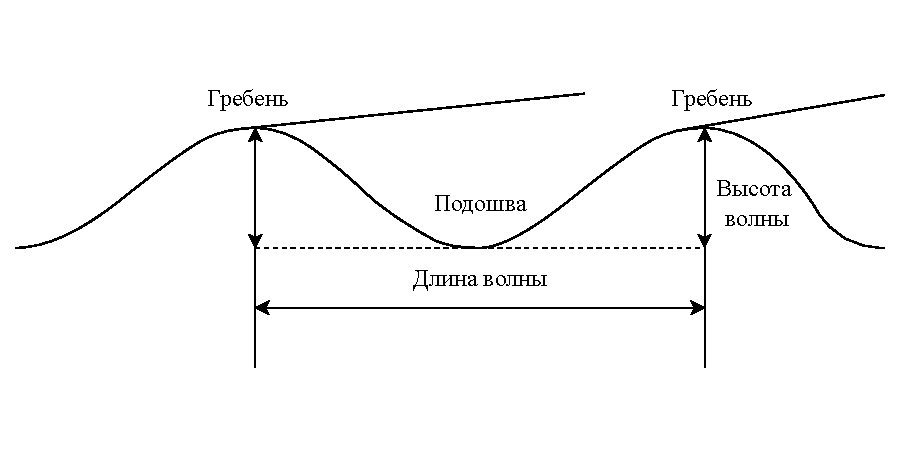
\includegraphics[scale=0.8]{img/wave.pdf}
	\end{center}
	\captionsetup{justification=centering}
	\caption{Геометрическое строение волны}
	\label{img:wave}
\end{figure}

По математическому описанию волны бывают линейные и нелинейные. Линейные волны обладают небольшой амплитудой, и их свойства описываются волновым уравнением для идеальной субстанции. Нелинейные волны обладают большой амплитудой, что изменяет математическую модель. Дисперсионные волны обладают линейностью.

В зависимости от требований к результату моделирования выбирается определенный метод визуализации. Так как в центре работы дисперсионные волны, для выполненения поставленных задач необходим такой метод моделирования, при котором выполняется дисперсионное соотношение --- корректно обрабатывается взаимодействие волны и объекта.

\section{Методы визуализации волн}

Существует три группы методов моделирования волн:

\begin{itemize}
    \item процедурные;
    \item методы на основе частиц;
    \item метод поля высот.
\end{itemize}

\subsection{Процедурные методы}

В процедурных методах для представления движения волн используются периодические функции. В ранних работах в качестве такой функции выступала циклоида \cite{orbit-procedure}, далее стали использовать синусоиду \cite{spectrum-darles}. Наложение периодических функций, изменяющихся во времени, создает волновую поверхность. Точка на такой поверхности описывает замкнутую круговую орбиту. Для создания различных волновых эффектов изменяют параметры уравнений орбиты, например, радиус, фазовый угол.

Процедурные методы чаще всего используют при визуализации масштабных волн океана. Преимуществом процедурного моделирования является возможность точно контролировать движение волнового спектра. Недостаток данных методов - сложность получения правильного взаимодействия волн с погруженными телами и границами.  

Выделяют следующие процедурные методы:

\begin{itemize}
    \item метод, основанный на модели Герстнера. Данный метод основан на решении уравнения Эйлера для гравитационных волн. Каждая частица на водной поверхности описывает окружность вокруг положения покоя. Тогда поверхность воды - кривая, которую описывает частица, находящаяся на расстоянии от центра окружности, которая катится по направляющей, как показано на рисунке 1.2. Эту кривую называют трохоидой. Используя лагранжевую систему отсчета находят все необходимые для визуализации параметры волн \cite{orbit-procedure};

\begin{figure}[H]
	\begin{center}
		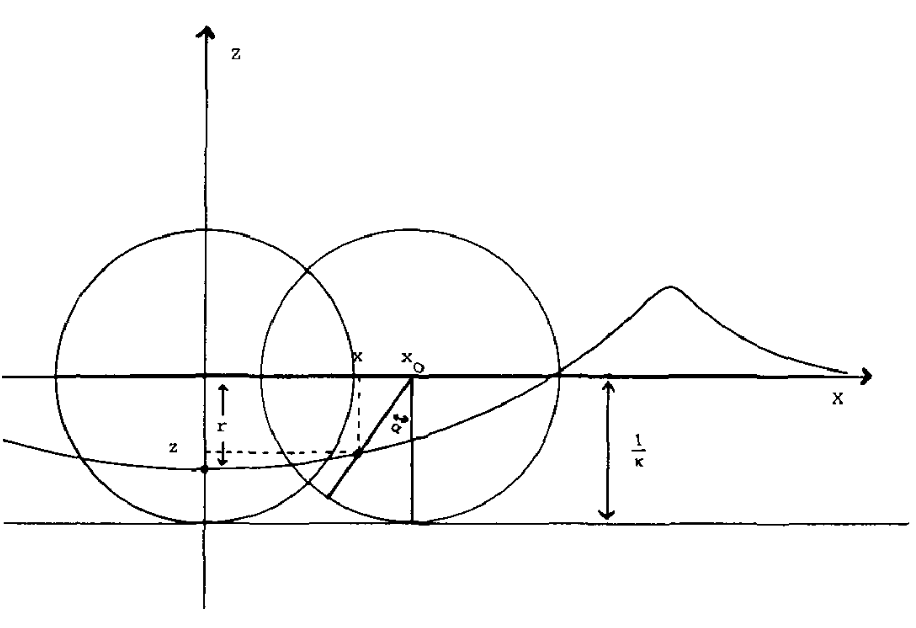
\includegraphics[scale=0.3]{img/trochoid.png}
	\end{center}
	\captionsetup{justification=centering}
	\caption{Поверхность воды представлена трохоидой.}
	\label{img:trochoid}
\end{figure}

    \item спектральные подходы. В данных подходах поверхность океана - поле высот, которое имеет спектр, соответствующий значениям реальной волновой поверхности. Генерируются синусоидальные волны, которые приближенно соответствуют реальным волнам. Если рассматривать функцию представления волны в частотной области, то можно добиться получения трохоид \cite{spectrum-darles}\cite{spectrum-tessendorf}.
\end{itemize}

\subsection{Методы на основе частиц}

В следующих методах моделирования волновой поверхности вода представляется как система частиц. Частицы движутся в соответствии с законами механики и обладают физическими величинами, т. е. задана функция. В определенный момент времени при помощи интерполяции можно получить значение этой функции в произвольной точке.

\begin{figure}[H]
	\begin{center}
		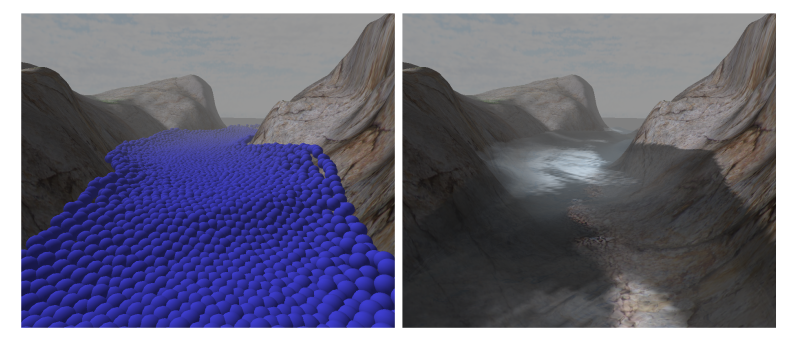
\includegraphics[scale=0.5]{img/particle.png}
	\end{center}
	\captionsetup{justification=centering}
	\caption{Поверхность воды представляется частицами (левый часть рисунка) и отображается в реальном времени (правая часть рисунка). }
	\label{img:particle}
\end{figure}

Для создания реалистичного изображения необходимо большое количество частиц, поэтому даннные методы используются при визуализации небольшого количества воды с неизвестной границей.   

Наиболее распространнёные методы на основе частиц:

\begin{itemize}
    \item гидродинамика сглаженных частиц (SPH). Метод SPH состоит из двух шагов: интерполяции объемов частиц в произвольных положениях и апроксимации пространственных производных. При интерполяции используется сглаживающая функция, называемая ядром, которая является кубическим сплайном. На результат интерполяции оказывают влияние только соседние точки, поэтому необходим поиск только соседних частиц. Так как частицы свободно перемещаются и перемешиваются в пространстве, встает необходимость эффективного решения задачи поиска соседних частиц. Тогда пространство разделяют на ячейки и суммируют по соседним ячейкам. Для большого объема жидкости данный метод создает нереалистичную поверхность \cite{sph};
    \item полунеявный метод движущихся частиц (MPS). Полунеявный метод движущихся частиц основывается на методе расчета движения жидкости Лагранжа. Уравнения движения жидкости дискретизируются с использованием движущихся частиц и их взаимодействий. Далее в методе MPS решается уравнение Навье-Стокса. При использовании данного метода существует возможность добавлять и удалять расчетные точки во время моделирования, поэтому метод является адаптивным. Одной из главных проблем данного метода является создание точных границ при контакте жидкости с твердым предметом или другой жидкостью \cite{mps}.
\end{itemize}

\subsection{Метод поля высот}

В случаях, когда визуализировать необходимо только поверхность воды, а не весь объем водоема, рассматривают волновое уравнение. Волновая поверхность представляется в виде двумерной функции - поля высот \cite{field}. 

Такое упрощение обладает важным преимуществом - снижением вычислительных затрат, что означает повышение скорости моделирования. Кроме того метод поля высот гибко обрабатывает препятствия. Но при такой модели в каждой точке поверхности известно только одно значение высоты, как это показано на рисунке 1.4. Это означает одинаковую скорость распространения всех волн, так, невозможно создать обрушивающиеся волны.

\begin{figure}[H]
	\begin{center}
		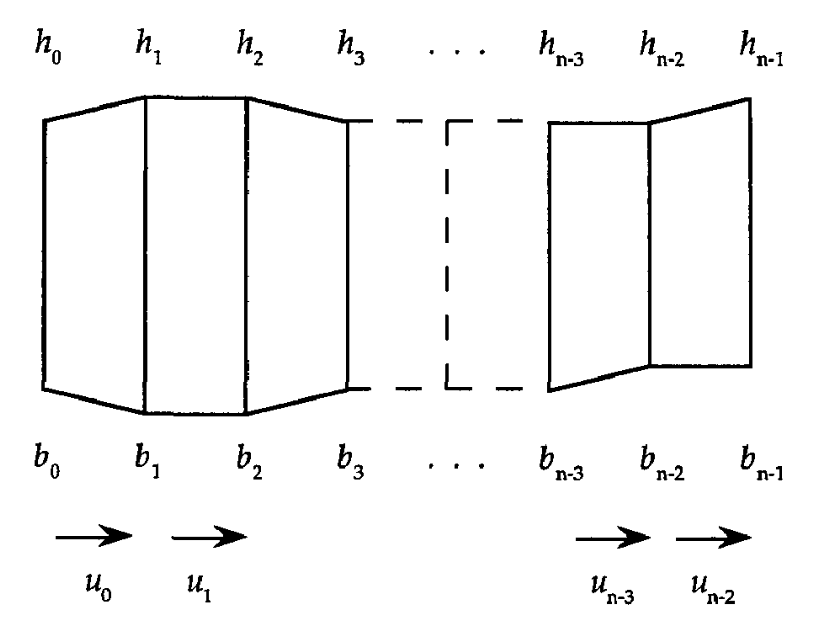
\includegraphics[scale=0.3]{img/height-field.png}
	\end{center}
	\captionsetup{justification=centering}
	\caption{Двумерное представление поверхности воды полями высот h с горизонтальной скоростью u и дна значениями b. }
	\label{img:height-field}
\end{figure}

Комбинация методов поля высот и методов, основанных на частицах, позволяет обходить недостатки отдельных и создавать различные эффекты \cite{shallow}\cite{large-small}.

\section*{Вывод}

Процедурные методы и методы на основе частиц имеют сложности при работе с твердыми телами. Метод поля высот корректно обрабатывает взаимодействие с объектом, причем с более высокой скоростью моделирования. Недостатки метода поля высот не имеют значения при решении выбранной задачи. Моделирование волн будет реализовано при помощи метода поля высот.

\section{Существующие программные обеспечения}

Одним из самых популярных программных обеспечений для работы с трехмерной компьютерной графикой является Blender \cite{blender}. Для моделирования жидкости, в том числе и волн, в Blender существует физическая среда с открытым исходным кодом - Mantaflow \cite{mantaflow}. Данный фреймворк может использоваться с графическим интерфейсом или без него в любой операционной системе. В этом программном продукте реализованы моделирование на основе уравнений Эйлера, гибкие системы частиц, моделирование жидкостей при помощи решателя FLIP, различные эффекты для жидкости, например, поверхностная турбулентность и вейвлет (небольшая рябь). На рисунке 1.5 показано моделирование гибкой системы частиц. 

\begin{figure}[H]
	\begin{center}
		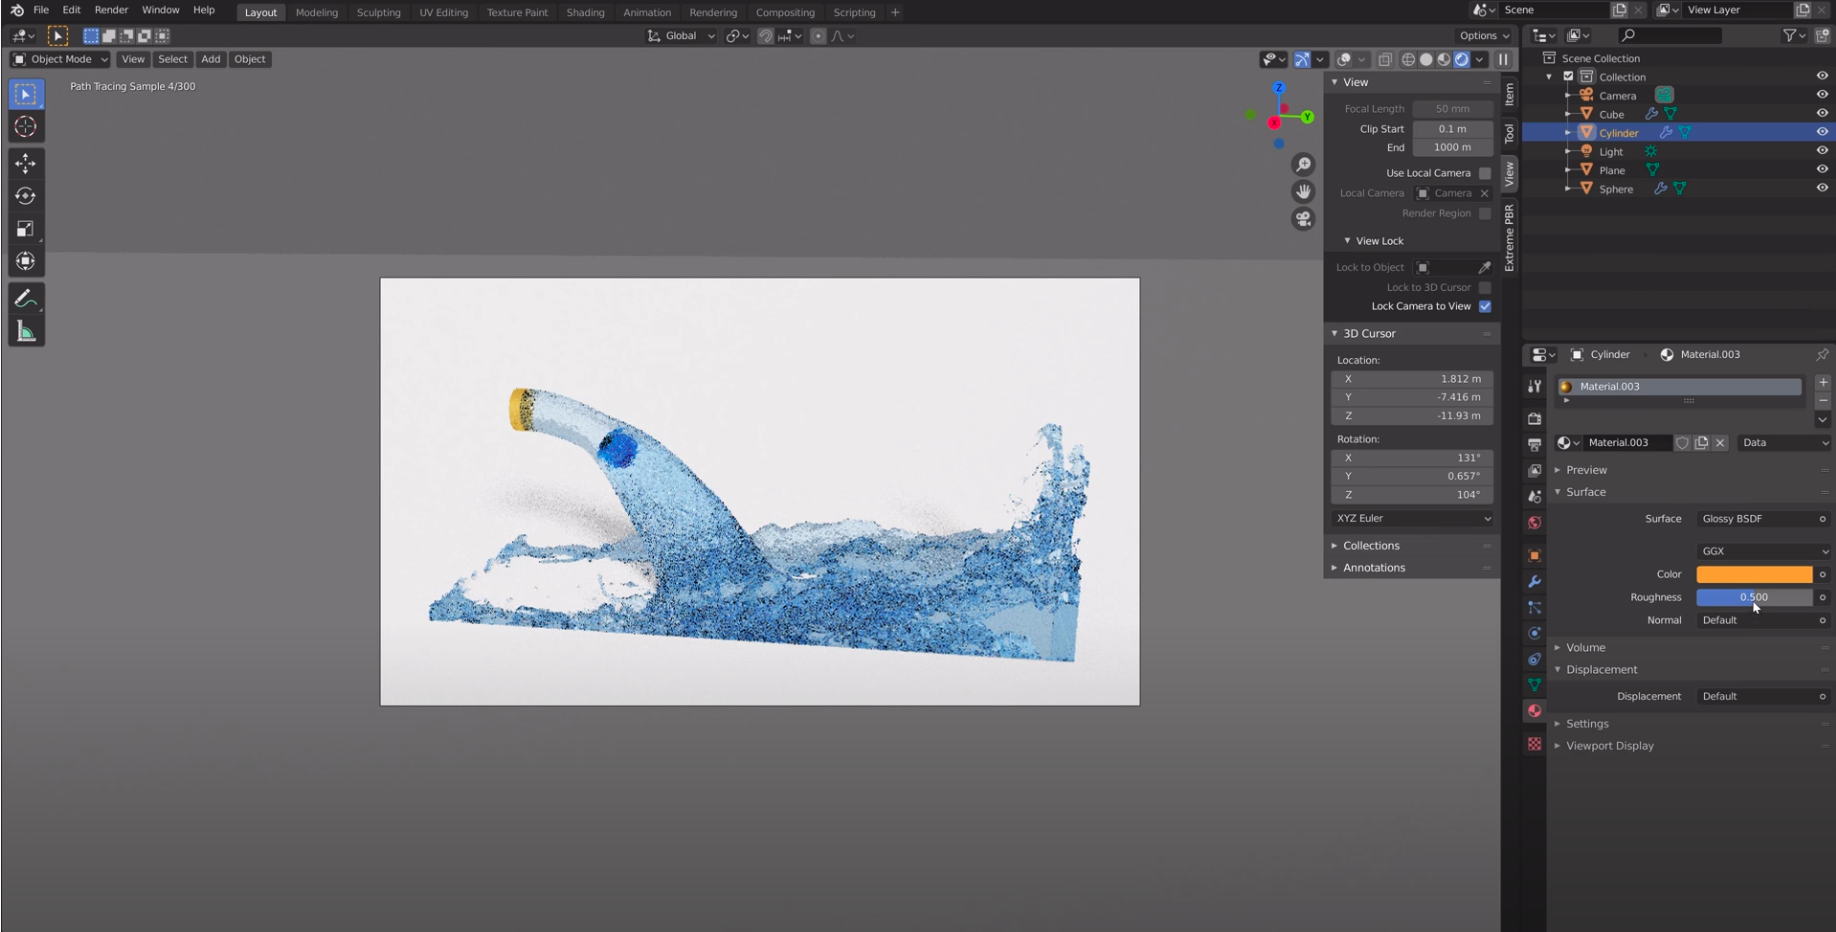
\includegraphics[scale=0.2]{img/mantaflow.png}
	\end{center}
	\captionsetup{justification=centering}
	\caption{Моделирование жидкости в среде Mantaflow в Blender.}
	\label{img:mantaflow}
\end{figure}

В коммерческих и научных проектах используются CFD пакеты. Например, FLOW-3D \cite{flow-3d} представляет набор инструментов для моделирования жидкостей, с целью исследования динамики их движения. Данный пакет позволяет моделировать линейные и нелинейные распространяющиеся поверхностные волны на основе метода конечных объемов. Для визуализации результатов используется программа визуализации FlowSight, как показано на рисунке 1.6.

\begin{figure}[H]
	\begin{center}
		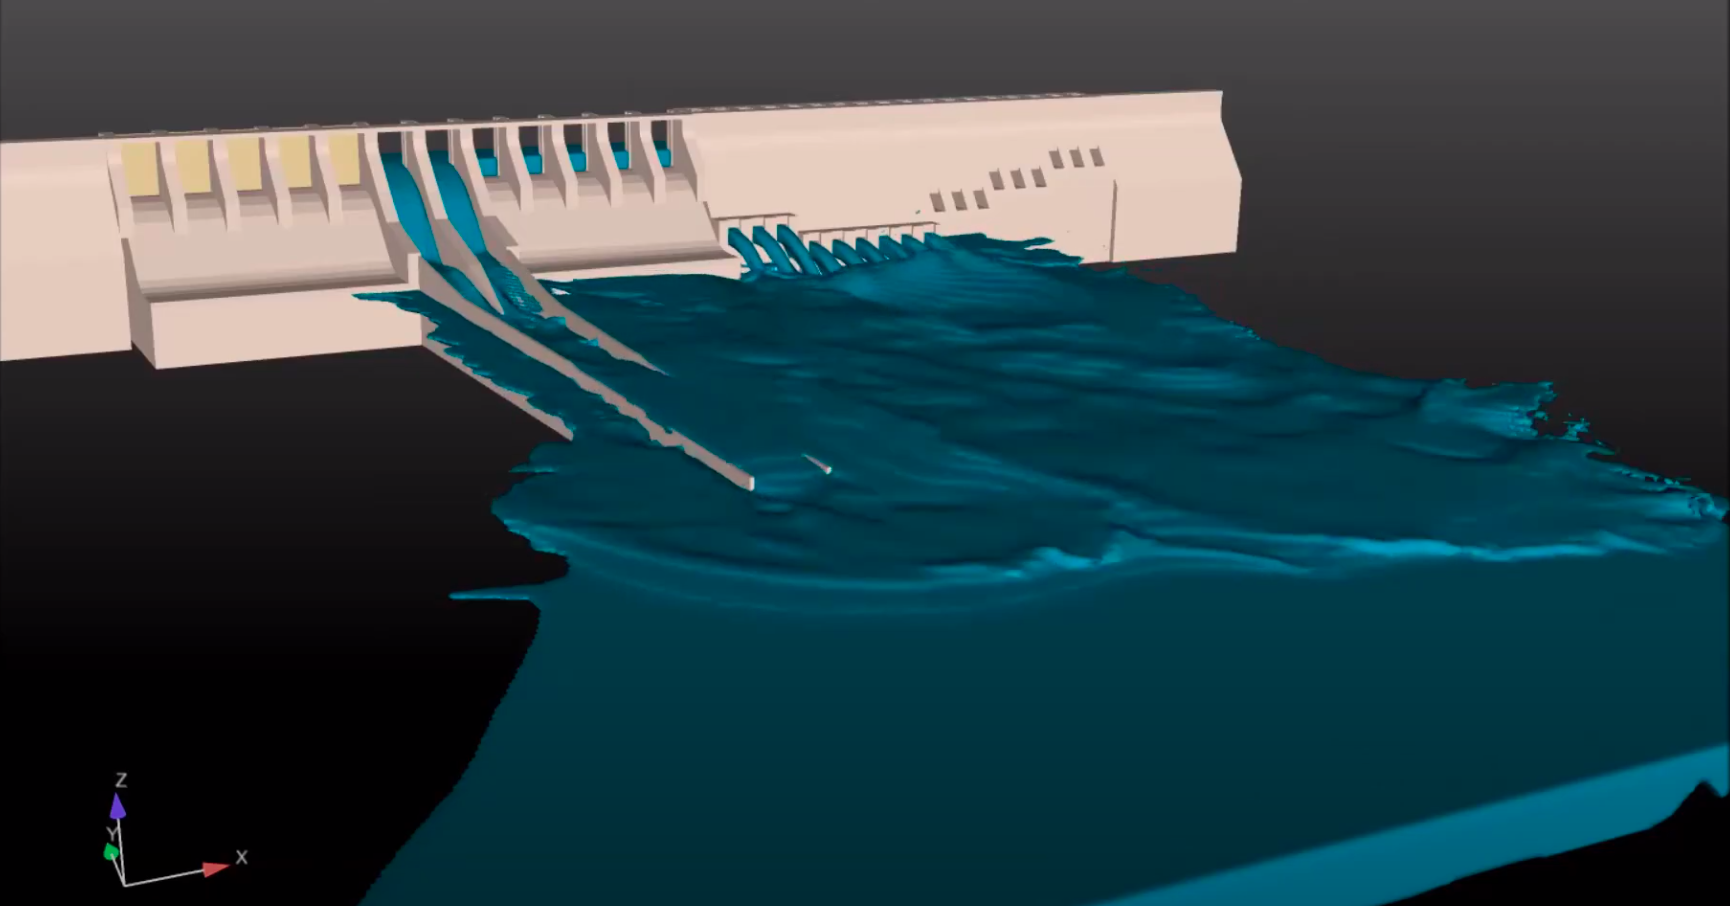
\includegraphics[scale=0.2]{img/flow-3d.png}
	\end{center}
	\captionsetup{justification=centering}
	\caption{Моделирование волн при помощи пакета FLOW-3D.}
	\label{img:flow-3d}
\end{figure}

\section*{Вывод}
